\documentclass[a4paper]{article}

\usepackage[english]{babel}
\usepackage[utf8]{inputenc}
\usepackage{amsmath}
\usepackage{graphicx}
\graphicspath{{/home/jorge/Imágenes/}}
\usepackage[colorinlistoftodos]{todonotes}
\usepackage{amsthm}
\usepackage{amssymb}
\usepackage{nccmath} 
\usepackage{verbatim}

\title{Teoría de Autómatas y Lenguajes Formales\\[.4\baselineskip]Práctica 1: Latex y expresiones regurales}


\author{Jorge Ramírez Zotano}

\begin{document}

\maketitle
                                                                                                                                
\section{Ejercicio }
\subsection{Definicion del automata}
Un Automata finito determinista (AFD) es un 5-tuple $(K, \Sigma, \delta,s, F)$ donde:\\
\begin{itemize}
\item $K$ es un conjunto no vacio de estados
\item $\Sigma$ es un alfabeto
\item $s \in K$ es el estado inicial
\item $F \subseteq K$ es un conjunto de estados finales
\item $\delta: K \times \Sigma \to K$ es una funcion de transicion
\end{itemize}
Entonces el automata requerido es:
\begin{itemize}
\item $K = \{q_{0},q_{1},q_{2}\}$ 
\item $\Sigma = \{a, b\}$ 
\item $s = q_{0}$ 
\item $F = \{q_{1}\}$ 
\item $\delta: $ \begin{table}[h!]
\begin{tabular}{c|c|c}
  $\delta(q,\sigma)$ & $a$ & $b$\\
  \hline
  $q_0$& $q_1$ & $q_2$\\
  \hline
  $q_1$& $q_2$ & $q_2$\\
  \hline
  $q_2$& $q_2$ & $q_2$
\end{tabular}
\end{table}

\end{itemize}
\subsection{Automata en JFLAP}

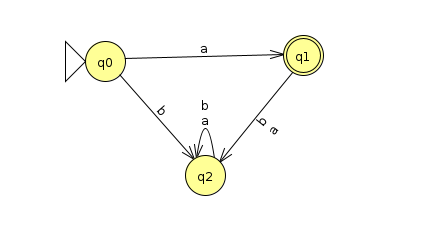
\includegraphics{Automata}

\subsection{Automata en Octave}

\verbatiminput{Automata_a.json} 

\end{document}